\documentclass[
11pt,%
tightenlines,%
twoside,%
onecolumn,%
nofloats,%
nobibnotes,%
nofootinbib,%
superscriptaddress,%
noshowpacs,%
centertags]%
{revtex4}
\usepackage{ljm}
\usepackage{listings}

\lstset{
language=C++,
basewidth=0.5em,
xleftmargin=45pt,
xrightmargin=45pt,
basicstyle=\small\ttfamily,
keywordstyle=\bfseries\underbar,
numbers=left,
numberstyle=\tiny,
stepnumber=1,
numbersep=10pt,
showspaces=false,
showstringspaces=false,
showtabs=false,
frame=trBL,
tabsize=2,
captionpos=t,
breaklines=true,
breakatwhitespace=false,
escapeinside={\%*}{*)}
}

\begin{document}

\titlerunning{dataflow processor emulator}
\authorrunning{Shabanov et al.}

\title{Features of Dataflow Processor Emulator Implementing}

\author{\firstname{B.~M.}~\surname{Shabanov}}
\email[E-mail: ]{shabanov@jscc.com}
\affiliation{Joint Supercomputer Center of the Russian Academy of Sciences -- branch of Scientific Research Institute of System Analysis of the Russian Academy of Sciences, Leninsky prospect 32a, Moscow, 119334, Russia}

\author{\firstname{E.~A.}~\surname{Kuznetsova}}
\email[E-mail: ]{mrallis@jscc.com}
\affiliation{Joint Supercomputer Center of the Russian Academy of Sciences -- branch of Scientific Research Institute of System Analysis of the Russian Academy of Sciences, Leninsky prospect 32a, Moscow, 119334, Russia}

\author{\firstname{A.~A.}~\surname{Rybakov}}
\email[E-mail: ]{rybakov.aax@gmail.com}
\affiliation{Joint Supercomputer Center of the Russian Academy of Sciences -- branch of Scientific Research Institute of System Analysis of the Russian Academy of Sciences, Leninsky prospect 32a, Moscow, 119334, Russia}

\firstcollaboration{(Submitted by A.~M.~Elizarov)} % Add if you know submitter.
%\lastcollaboration{ }

\received{May 01, 2020; revised May 30, 2020, accepted June 05,
2020}

\begin{abstract}
The development of dataflow processor architecture is a promising
direction for improving the performance of computing systems. The
dataflow processors have several advantages in contrast with the von
Neumann architecture processors. These advantages are express in
explicit parallelism of calculations, since in the presentation of
programs for the dataflow processors the execution of instructions
is limited solely by the fact of input data's ready state. The
concept of using tokens as data storage for instructions allows you
to remove many problems associated with data conflicts and
simplifies the program logic. One of the most important elements in
the implementation of the logic of the dataflow processor is the
associative token memory, which should provide storage and quick
search for ready-made data for instructions that can be transferred
for execution. This article discusses the functionality of the
dataflow processor emulator and its parts including associative
token memory and the logic of its operation using the example of a
simple dataflow graph.
\end{abstract}

\subclass{68N20,68R10} % Enter 2010 Mathematics Subject Classification.

\keywords{Dataflow processor emulator, dataflow graph, token, token state, associative token memory, control flow graph, def-use graph.}

\maketitle

\section{Introduction}

A processor with dataflow architecture (dataflow processor) has the potential to provide the highest performance among processors due to the fact that the parallelism of command execution is taken into account when drawing up a program graph.
The program execution is not required to be performed by sequentional translating of the sequence of instructions, as is in the case of a processor with the von Neumann architecture.
A program in the dataflow processor is a directed graph where nodes are instructions, and information transfers by the edges as tokens, which contains the data field and context field of transferring data.
This context identifies where token should be sent to (the identifier of command and number of its argument) and also contains the state, which allows executing different iterations of nested loops and different executions of procedures at the same program graph at parallel.
And regardless of the place of the instruction with many inputs in the graph, it is passed for execution when the last of the operands (tokens) with the same state arrived.
After calculating the result of the instruction, new tokens with the result value are sent to the inputs of subsequent commands according to the program graph, and the used operand tokens are destroyed.

At the same time, in contrast to the von Neumann architecture, the dataflow processor has not a central control device (and instruction counter), and the parallelism of the executing instructions is determined in dynamics by the arrival of operands to the instruction inputs in the decentralized scheme.
Namely, the device for searching ready-to-execute commands -- the memory of searching arguments sets (the token assiciative memory) can be executed such as many parallel-running modules, which provides the same large numbers of arithmetic, logic or vector execution units.
Since the execution of an instruction is dependent upon the arrivals of operands, the management of token storage and instruction scheduling are intimately related in any dataflow processor \cite{fine-grained-prl,culler}.

Unlike the implementation of a multiprocessor system, direct hardware implementation allows you to fully implement the calculation graph in the form of a computing pipeline, thereby eliminating the need to create a module that implements the execution of the calculation schedule \cite{popov}.

The difficulties noted above for the hardware implementation of the dataflow processor led to the fact that none of the many projects for its creation was possible to achieve higher performance compared to the von Neumann processor, and by the end of the 2000s, there were practically no such projects.
This refers to the development of universal dataflow processors, but not specialized ones, since, for example, dataflow processors of digital signal processing were not only developed, but also produced \cite{terada}.

The Joint Supercomputer Center of the Russian Academy of Sciences (JSCC RAS) is developing a vector processor with the dataflow architecture \cite{vpp}.
This paper introduces the development of the emulator of the model of dataflow processors family.


\section{Emulation of processor with the von Neumann architecture}

One of the basic principles of the von Neumann architecture is the principle of control flow.
According to it, the executable code of the program is stored in memory, and the processor can execute its instructions sequentially, one by one.
The next instruction address submitted to the processor for execution is stored in a special register called instruction pointer.
By default, it always shifts to the next instruction in memory.
This address can be forcedly changed by special transition instructions, and in this case, we can talk about transferring control to another part of the program.

Let's introduce the concept of a linear section (or program basic block).
The linear section is a sequence of instructions with the next two properties.
First, control could only be transfered to the first instruction of a given section.
In other words, a linear section has only one input, which is the section's first  instruction.
Second, if control was transferred to the linear section, then all instructions of this section must be executed (i.e., there can be no transition instructions inside the linear section).
The transition instruction can only be at the end of the linear section.
Sometimes, instead of linear sections, it is convenient to view so-called quasilinear sections, which can have an arbitrary amount of transition instructions inside for transitions to other linear sections.
We will not consider quasilinear sections, because any such section can be divided into a sequence of ordinary linear sections.

An important concept widely used in the theory of optimizing compilers is the control flow graph (CFG) \cite{Muchnick}.
A control flow graph is a directed graph whose nodes are linear sections of the program, and edges indicate the transfer of control between them.
The control flow graph is a convenient and demonstrative structure for describing program behavior and used by optimizing compilers to implement global program optimizations, i.e. optimizations that operate with linear sections.

Consider the logic of intermediate program representation inside one linear section.
Consider for this a simple example of finding the roots of a quadratic equation.
We will use listing in the C programming language to write examples and pseudocode.
Thus, we have a linear section (program code block) at the input of which we have the variables $a$, $b$, $c$ containing the coefficients of the quadratic equation $ax^2 + bx + c = 0$.
At the linear section output it is required to get the values of the roots, which are calculated by the common formulas $x_{1,2} = (-b \pm \sqrt{b^2 - 4ac})/(2a)$.

\begin{lstlisting}[caption={Code block for calculating the roots of quadratic equation.},label={lst:square_equation_1}]
{
    float t = sqrt(b * b - 4.0 * a * c);

    x1 = (-b + t) / (2.0 * a);
    x2 = (-b - t) / (2.0 * a);
}
\end{lstlisting}



In listing~\ref{lst:square_equation_1}, the linear section is highlighted by curly brackets and temporary variable $t$ is declared to understand that this variable is not used outside the linear section.
For convenience, we assume that the processor, for which the executable code will be created, supports the instruction for calculating the square root.
Thus, the following instructions for working with real numbers appear in the listing above: MUL is a multiplication of two numbers, SUB is a subtraction of two numbers, SQRT is a square root of a number, NEG is an unary negative, ADD is an addition of two numbers, DIV is a division of two numbers.

\begin{figure}[h]
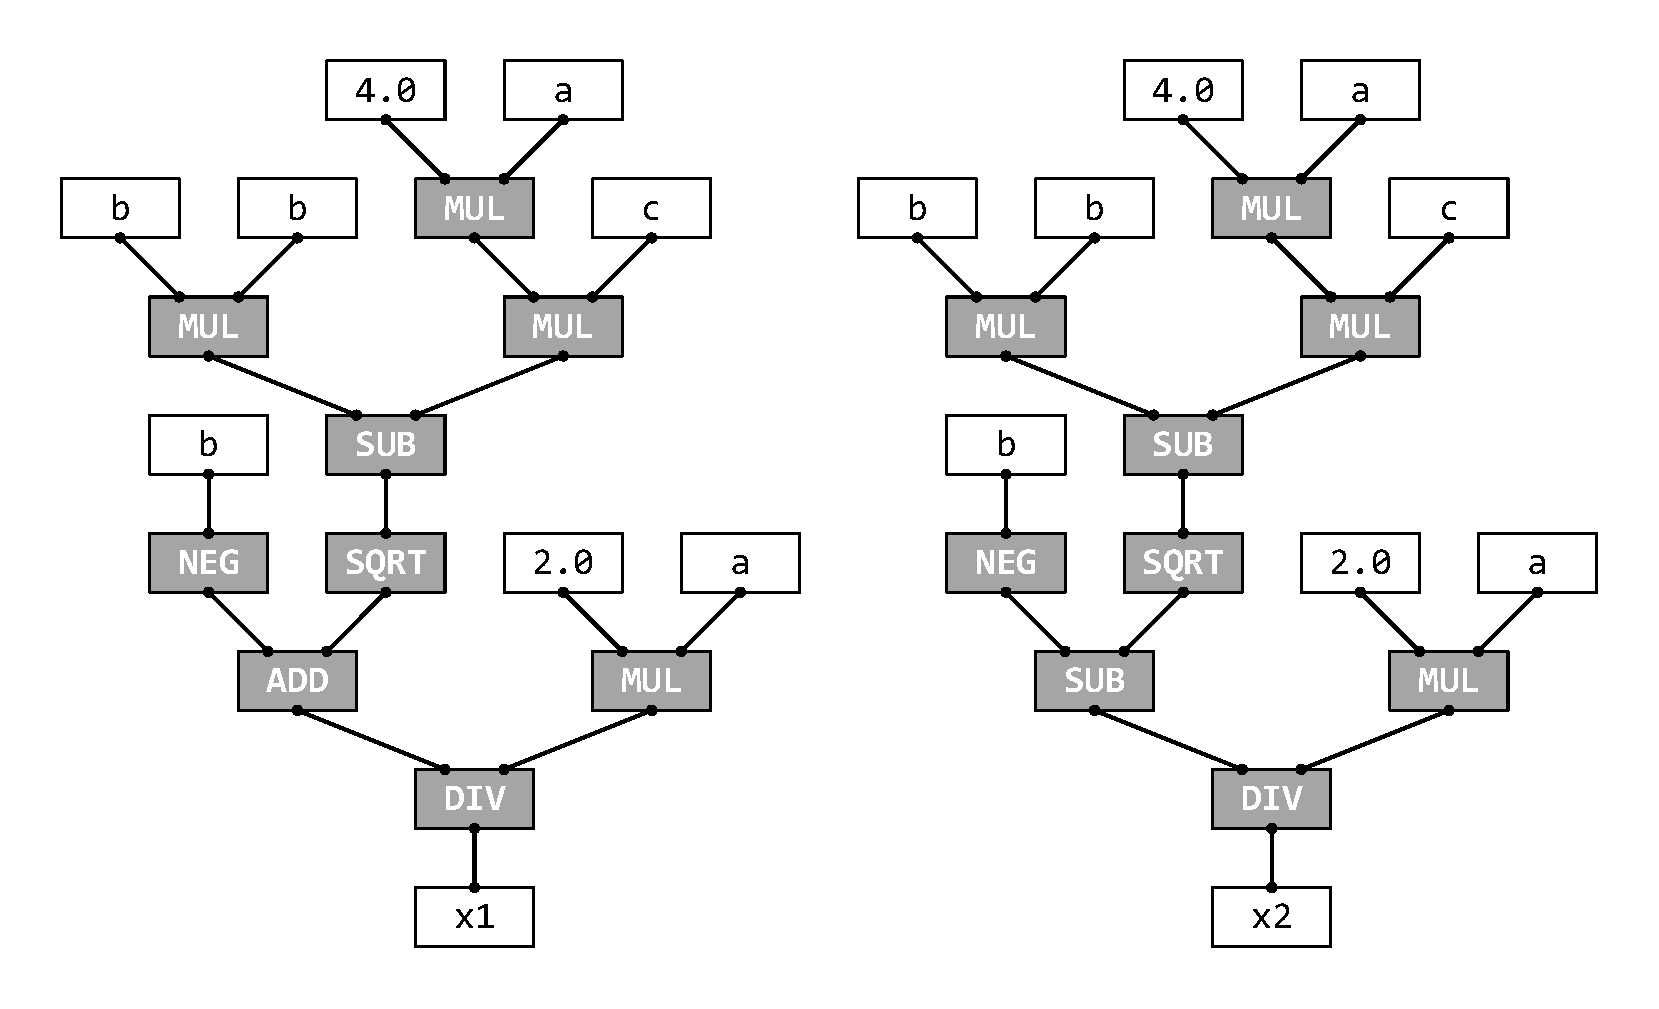
\includegraphics[width=0.75\textwidth]{pics/square_equation_calculation_tree.pdf}
\captionstyle{center}\caption{Trees for calculating the roots of quadratic equation.}\label{fig:square_equation_calculation_tree}
\end{figure}

Figure~\ref{fig:square_equation_calculation_tree} shows two trees of evaluating the expressions $x_1$ and $x_2$.
The compiler, of course, will simplify the calculation data by collecting common subexpressions, and the final version of the linear section representation will be close to the dependency graph shown in Figure~\ref{fig:def_use} (def-use graph, DFG).

Nodes of this directed graph are separate operations (shown as dark rectangles), and edges are def-use dependencies between data operations (the $B$ command depends on the $A$ command if uses the data generated by the $A$ command).
It can be other kinds of dependencies between operations besides data dependency (control dependency, anti-dependency), but these types of dependencies are missing in our simple example.

To form the resulting executable code the presence of a def-use graph is not enough.
It is necessary to line up all commands included in the def-use graph in a single sequence, which will subsequently be written to a linear section of memory.
In this case, when aligning a sequence of commands, it is necessary to observe the requirement that if the $B$ command depends on the $A$ command according to the data, then it should be later than the $A$ command in the final sequence.
This process called code planning \cite{Aho}.
In the result of code planning in the considered case, we will get a pseudocode for calculating the roots of quadratic equation similar to the code in listing~\ref{lst:square_equation_2}.



\begin{lstlisting}[caption={Pseudocode for calculating the roots of  quadratic equation.},label={lst:square_equation_2}]
MOV 4.0       ->  v0
MOV   a       ->  v1
MOV   b       ->  v2
MUL  v0,  v1  ->  v3
MOV   c       ->  v4
MUL  v3,  v4  ->  v5
MUL  v2,  v2  ->  v6
NEG  v2       ->  v7
SUB  v6,  v5  ->  v8
SQRT v8       ->  v9
MOV 2.0       -> v10
MUL v10,  v1  -> v11
ADD  v7,  v9  -> v12
SUB  v7,  v9  -> v13
DIV v12, v11  -> v14
DIV v13, v11  -> v15
MOV v14       ->  x1
MOV v15       ->  x2
\end{lstlisting}

\begin{figure}[h]
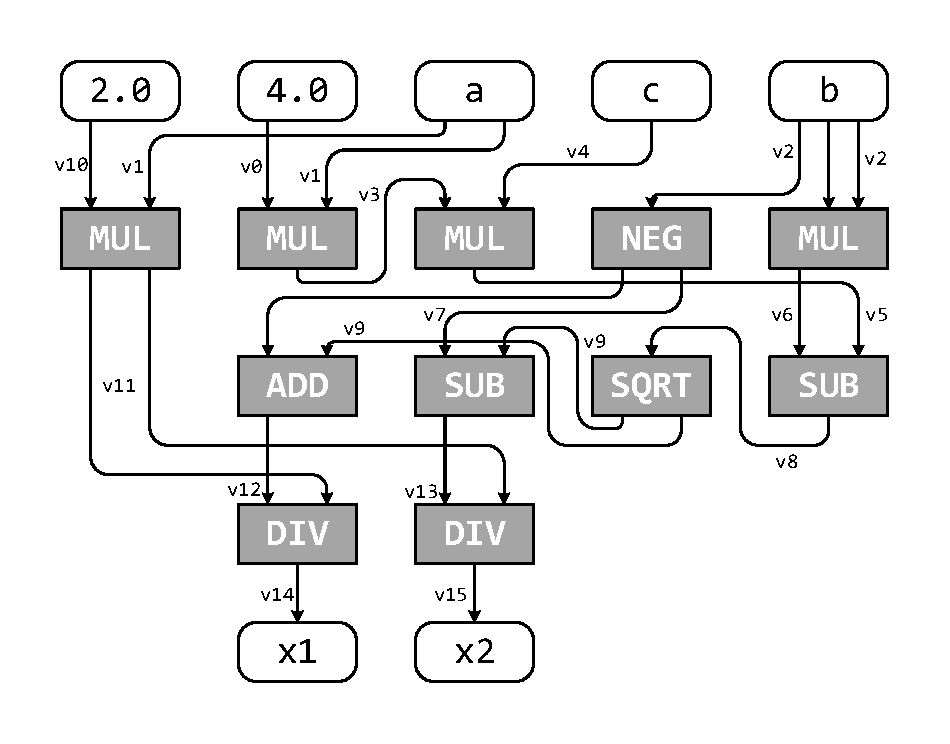
\includegraphics[width=0.45\textwidth]{pics/def_use.pdf}
\captionstyle{center}\caption{Dependency graph of a linear section which calculates the roots of quadratic equation.}\label{fig:def_use}
\end{figure}

In Listing~\ref{lst:square_equation_2}, all instructions except transmission operation operate on virtual registers (v0-v15).
The order of the commands is important in this form.
At any time after the execution of any instruction, we can talk about some state of the processor which is characterized by the content of memory and of all the registers used.

The main part of the processor emulator is the realization of instruction semantic, executed by the processor.
Every instruction is considered as a function, which transfers the computer from one state to another.

\section{Dataflow processor emulation}

The dataflow processor emulator, which considered in this article,
has a dynamic model. It permits to pass the commands for execution
when their tokens are ready with the simultaneous execution
possibility of inner cycle' iterations and different procedure
launches on the same program graph.

The dynamic model of the dataflow processor allows revealing more parallelism in program due to not only the coincidence of command number, of the operand tokens, but also of the tokens state \cite{Wiley}.

In contrast with processors with the von Neumann architecture, dataflow processors do not need complete orderliness in command execution.
I.e. if two instructions can be executed in parallel (this is possible in the absence of dependence between them) then the order of their execution is not determined.
We will consider the same example of the linear section, inside which the roots of the quadratic equation are calculated.
The program for the dataflow processor is the graph just like the def-use graph showed in Figure~\ref{fig:def_use}.
Dataflow graph, which is a program for dataflow processor, is also directed.
The nodes of this graph are also the instructions, but edges have a completely different meaning.
In the case of def-use graph, edges were fixed fact of the dependence between two operations (indicating by which variables, by which resource), in case of dataflow graph the edge is a unique data carrier that names token.
Therefore, the token is a data structure that stores information about transferring data and about the destination point of this data (the identifier consuming this instruction data as well as the argument number).
Besides, the token contains additional information (token state) allowing to distinguish instruction, which relates to different function calls or to different loop iterations, but for this example, this is not important, therefore, the description of token state will be omitted.

\begin{figure}[h]
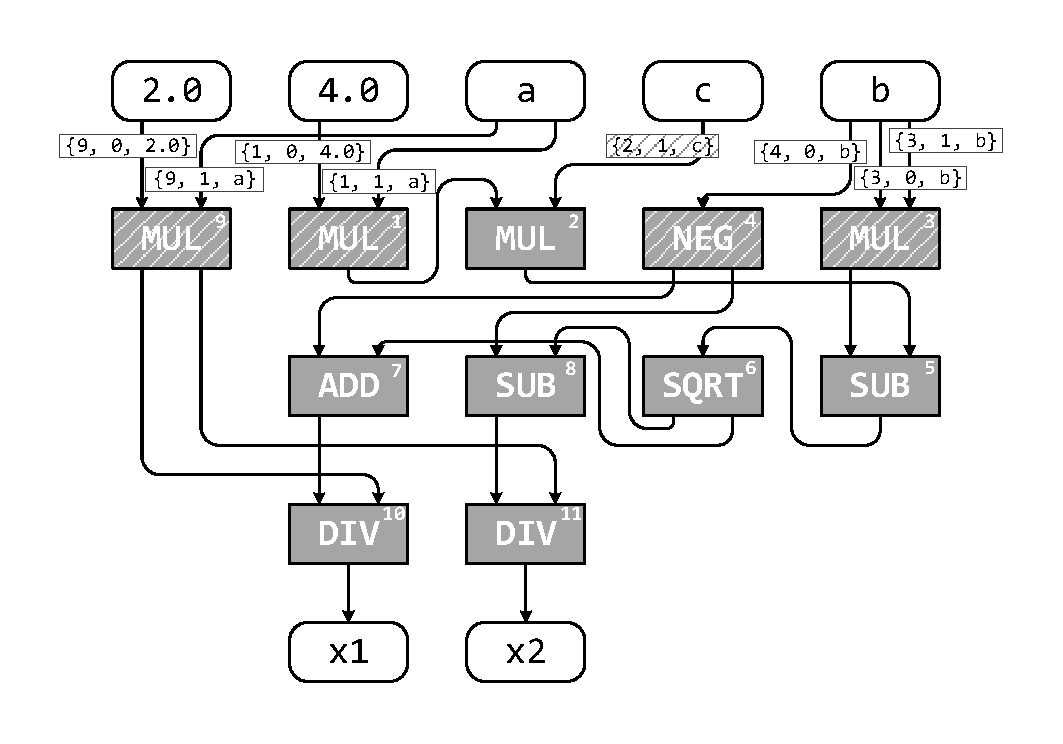
\includegraphics[width=0.5\textwidth]{pics/dataflow.pdf}
\captionstyle{center}\caption{Dataflow graph of a linear section which calculates the roots of a quadratic equation.}\label{fig:dataflow}
\end{figure}

Figure~\ref{fig:dataflow} shows the dataflow graph in the initial time when none of the instructions have been completed yet.
In this figure, on the edges of the graph, you can see those tokens that are ready and transferred to the relevant instructions.
For example, for the instruction 9 MUL two tokens are ready: $\{9, 0, 2.0\}$ (9 is a number of instruction, 0 is number of a argument, 2.0 is a real number), $\{9, 1, a\}$ (9 is a number of instruction, 1 is a number of argument, $a$ is a real number).
Both arguments for the instruction 9 MUL are ready and instruction can be executed.
After execution, tokens containing arguments are deleted, and tokens containing the result of instruction 9 MUL will be sent by the output edges to instructions 10 DIV and 11 DIV.

If we consider another instruction 2 MUL, we can see that only the second argument is ready for it (token $\{2, 1, c\}$).
The first argument will only be generated after executing the 1 MUL instruction.

Thus, all instructions in the presented graph will be processed until the required values are obtained in tokens on the output edges from instructions 10 DIV and 11 DIV.

The implementation of instruction semantics in a dataflow processor emulator is no different from the same functionality in a traditional processor emulator.

The central functional element for ensuring the operability of the dataflow processor is so-called associative token memory, which is designed to store and search tokens for ready-to-execute commands.

Associative token memory is a repository of tokens that are
currently created and are being executed in the program. Moreover,
if it turns out that in the associative memory there are all the
necessary arguments for a command, they are immediately removed from
the associative memory and sent for execution to the command. Thus,
at any moment in time in the associative memory there are only those
arguments that wait for the missing arguments for some instructions.
That is, at the conditionally first moment in time, shown in the
Figure~ \ref{fig:dataflow}, in the associative memory of tokens
there is only one token $\{2, 1, c\}$, waiting for its pair, while
the commands are 9 MUL, 1 MUL, 4 NEG, 3 MUL are already ready for
execution and are in the command buffer along with sets of their
arguments.

The dataflow processors approach resolves any threads of control into separate instructions that are ready to execute as soon as all required operands available \cite{silc}.
In the Figure~\ref{fig:dataflow} the token located in the associative memory is shaded, as well as the commands ready to be executed.

\begin{figure}[h]
\setcaptionmargin{5mm} % if the caption is multiline
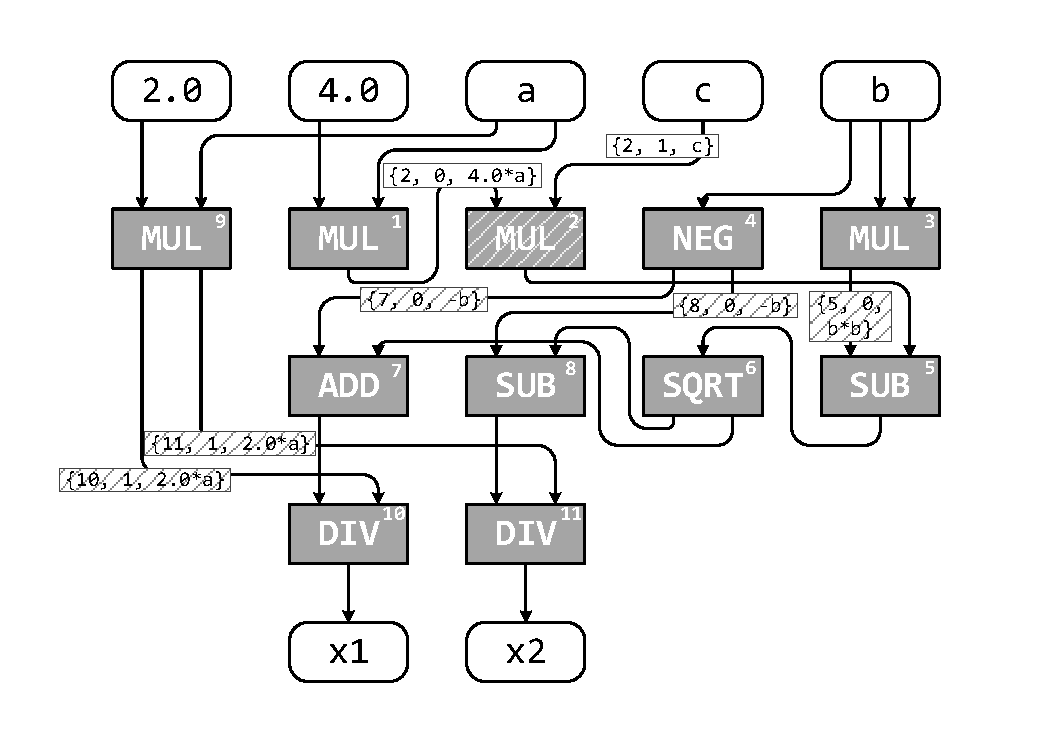
\includegraphics[width=0.50\textwidth]{pics/dataflow2.pdf}
\captionstyle{center}\caption{Dataflow graph of a linear section which calculates the roots of quadratic equation before executing the 2 MUL instruction.}\label{fig:dataflow2}
\end{figure}

After execution of the instructions 9 MUL, 1 MUL, 4 NEG and 3 MUL,
the only instruction ready for execution is 2 MUL. The state of the
computer before executing this instruction is shown in the Figure
~\ref{fig:dataflow2}. In this figure, the 2 MUL instruction ready
for execution is visible, as well as several tokens that have been
passed into associative memory. Further execution of the program is
similar and at the end we come to the formation of two tokens on the
output edges of operations 10 DIV and 11 DIV, which will then be
sent to their consumer instructions.

In the dataflow processors, overflow of the associative memory is unacceptable, that is why the associative memory must have high capacity and be fast at the same time, which is difficult to realize in practice.
That is the point to implement the emulator, which will help to get closer to creating such the dataflow processor while revealing all possible errors and shortcomings.

\section{Architecture of dataflow processor emulator}

Consider the architecture of the dataflow processor emulator in general, presented in Figure~\ref{fig:big-scheme}.

\begin{figure}[h!]
\center{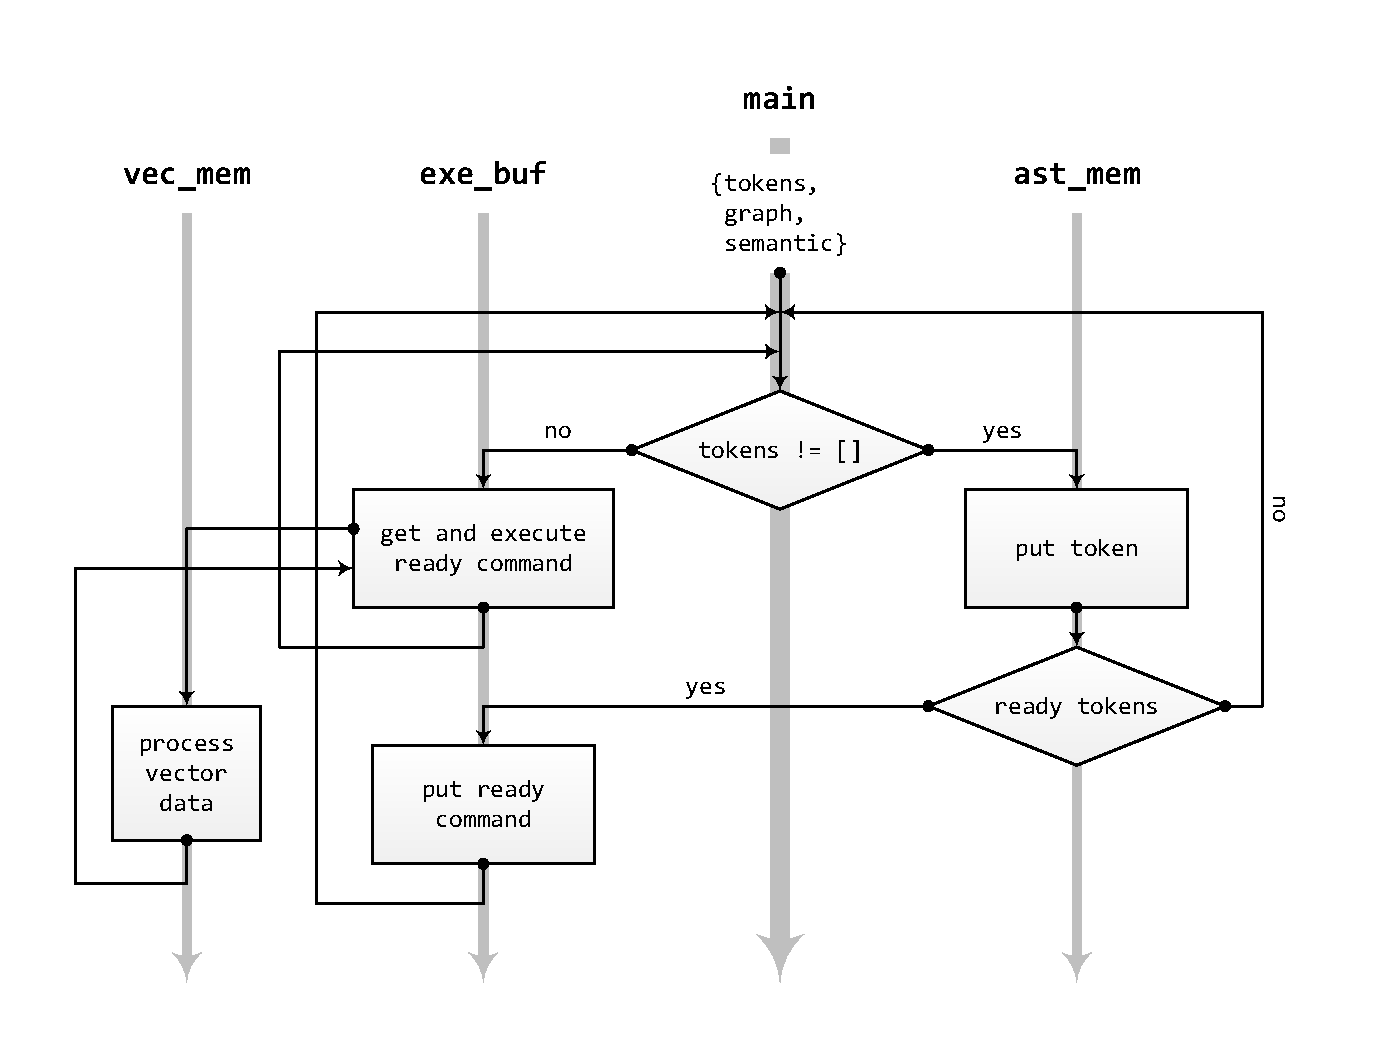
\includegraphics[width=0.8\textwidth]{pics/big-scheme2.pdf}}
\captionstyle{center}\caption{General architecture of dataflow
processor emulator.} \label{fig:big-scheme}
\end{figure}

The vector dataflow processor emulator is implemented using four infinite processes that exchange messages with each other.
Each process is a separate processor entity and has its own functionality.

The main process $main$ is the lead in the emulator.
He is the host of three basic data structures that reflect the execution of the program.
The $tokens$ structure contains a list of tokens that currently exist during program execution.
The structure of $graph$ is a directed graph that implements the logic of the program.
Finally, the $semantic$ structure describes the semantics of processor instructions, that is, it contains the implementation of functions that, according to a set of input tokens, generate sets of output tokens for each instruction.

The next process under consideration is the $ast\_mem$ process, which implements the logic of associative token memory.
The interface of this process consists of one single function -- to put a token into associative memory.
In the event that this token is the last missing element for executing any instruction, then the entire set of input tokens for this instruction is deleted from the associative token memory and transferred to form a command that is ready for execution.

For storage of ready-to-execute commands, the process $exe\_buf$ is intended.
This process is a simple queue containing all currently ready commands.
Accordingly, in this queue, you can add a command along with its ready token arguments, or you can get some command and remove it from the queue.

To implement the work with vector arguments of commands, a vector storage is intended, which is implemented using the $vec\_mem$ process.
Work with this repository is carried out using the vector address.
The vector memory interface consists of such requests as: allocate a new vector, get a vector from memory, get a vector element, write a specific value to a vector element, etc.

The logic of the emulator consists of an endless poll of the head process $main$.
At each iteration of the survey, the following logic for processing data structures $tokens$, $graph$ and $semantic$ is performed.
If the $tokens$ structure contains tokens, then one of them is taken and sent to $ast\_mem$.
After that, depending on the response of the process $ast\_mem$, the token can simply be added to the associative tokens memory, or a ready-to-execute command can be generated and placed in the buffer $exe\_buf$.
If the structure $tokens$ is empty, then the head process receives the first (or arbitrary) command from the ready-made instructions buffer and executes it using the semantics storing in $semantic$ structure.
Next, the generated tokens of the result of the executed command with the help of the $graph$ structure receive information about the destination commands and are added to the $tokens$ structure.
After that, the program execution cycle continues again until the target tokens are received and the buffer of ready-to-execute instructions is empty.

The described logic of the interaction of the processes of the emulator of a dataflow processor is implemented using the Erlang programming language \cite {Armstrong, Cesarini}.
Erlang programming language is a functional language designed to implement separate parallel processes that exchange messages.
Messaging between processes is the only way to ensure communication between processes (the language does not have the concept of shared memory) it is supported at the syntactic level.
Parallel to the execution of processes is a natural behavior of the language; therefore, it is not necessary to implement additional tools to ensure the interaction of system elements.

\section{Conclusion}

The article discusses the differences in the implementation of an executable program designed for a processor with von Neumann architecture and for a dataflow processor.
The differences between the def-use graph and the dataflow graph are shown, which reflect the program logic within the linear section.
A dataflow processor emulator implementation is considered, including associative token memory, with which it is possible to store and quickly find ready-made data for commands that can be transferred for execution.
This dataflow processor emulator architecture can be used for implementing dataflow processor with arbitrary logic and semantic of instructions.
This approach to dataflow processor emulator is used in the emulator implementation of a vector dataflow processor which is being developed at the JSCC RAS.

\begin{acknowledgments}
The work has been done at the JSCC RAS as part of the state assignment for the topic 0065-2019-0016 (reg. no. AAAA-A19-119011590098-8).
The supercomputer MVS-10P, located at the JSCC RAS, was used during the research.
\end{acknowledgments}

\begin{thebibliography}{99}

\bibitem{fine-grained-prl}
\refitem{article} N.~A.~Dikarev, B.~M.~Shabanov, and A.~S.~Shmelev,
{\it ``The use of fine-grained parallelism in dataflow processor"},
Problems of developing promising micro- and nanoelectronic systems
(MES) {\bf 2}, 144--150 (2016).

\bibitem{culler}
\refitem{book}
D.~Culler, {\it ``Dataflow Architecture"}, MIT/LCS/TM-294, Massachusetts Institute of Technology (1986).

\bibitem{popov}
\refitem{article} R.~I.~Popov, {\it ``Application of stream computer
models in designing specialized processors"}, Scientific and
Technical Journal of Information Technologies, Mechanics and Optics
{\bf 5} (75), 77--81 (2011).

\bibitem{terada}
\refitem{article} H.~Terada, {\it ``DDMP's: Self-Timed
Super-Pipelined Data-Driven Multimedia Processors"}, Proceedings of
the IEEE {\bf 2} (86), 282--296 (1999).

\bibitem{vpp}
\refitem{article} N.~A.~Dikarev and B.~M.~Shabanov, {\it ``Vector
dataflow processor"}, IZVESTIYA SFedU {\bf 10} (54), ~80--85 (2005).

\bibitem{Muchnick}
\refitem{book} S.~S.~Muchnick, {\it ``Advanced Compiler Design \&
Implementation"}, Academic Press (1997).

\bibitem{Aho}
\refitem{book} A.~V.~Aho, M.~S.~Lam, R.~Sethi, and J.~D.~Ullman,
{\it ``Compilers. Principles, Techniques, \& Tools"}, Addison-Wesley
(2007).

\bibitem{Wiley}
\refitem{book}
J.~Wiley, {\it ``Dataflow Computers: Their History and Future. \& Wiley Encyclopedia of Computer Science and Engineering, edited by Benjamin War"}, John Wiley and Sons, Inc (2008).

\bibitem{silc}
\refitem{book} J.~Silc, B.~Robic, and T.~Unqerer, {\it ``Processor
Architecture: From Dataflow to Superscalar and Beyond"}, Springer
Science and Business Media (2012).

\bibitem{Armstrong}
\refitem{book}
J.~Armstrong, {\it ``Programming Erlang. Software for a Concurrent World."}, Pragmatic Programmers (2013).

\bibitem{Cesarini}
\refitem{book} F.~Cesarini and S.~Thompson, {\it ``Erlang
programming."}, O'Reilly (2009).

\end{thebibliography}

\end{document}
